\chapter{Improving SAT-to-QUBO}
\label{cha:QAcore}

This chapter will first discuss the weaknesses of the current SAT-to-Ising definition approach, later suggesting a novel algorithm to refine the encoding and retrieve a more stable solution. 

\section{Algorithm}

The goal of postprocessing is the re-definition of the QUBO encoding, modifying offset, biases and couplings between qubits so that the longer chains are reduced in size. Since all nodes that make up the chain are linked by couplings whose value is $-1$, we will ensure to modify these weights. \\
The only way to achieve this task while not altering the original SAT formulation is to re-compute the scores of each chunk of the simplified formula, defining new OMT problems that involve the additional qubits. In more details, given two penalty functions encoded in a quantum annealer architecture linked by a chain:

\begin{itemize}
    \item We split the chains into two disjoint sets of nodes. The first set will be associated to the first penalty function, the second to the other.
    \item We use nodes composing the original penalty functions and the newly assigned qubits of the chain to calculate again the weights of. In particular, we use the nodes belonging to the chain as ancillas for the new function, forcing each coupling between chain nodes and penalty function qubits to be different from zero. We need also to set the most external node of the chain as the actual shared variable, so that we ensure that there is a way to link qubits representing the same Boolean variable and enforcing their equality.
    \item At this point, we have obtained a subgraph of the original architecture referring to the same. To compute new weights for, we will again rely on formula, but the presence of new ancillas will help us in reducing the number of coupling with score -1. These weights are then used to modify the QUBO encoding before being passed as input to the annealer.
\end{itemize}

A graphical representation of the algorithm is shown in figure 4.1.
\begin{figure}[b!]
	\begin{center}
	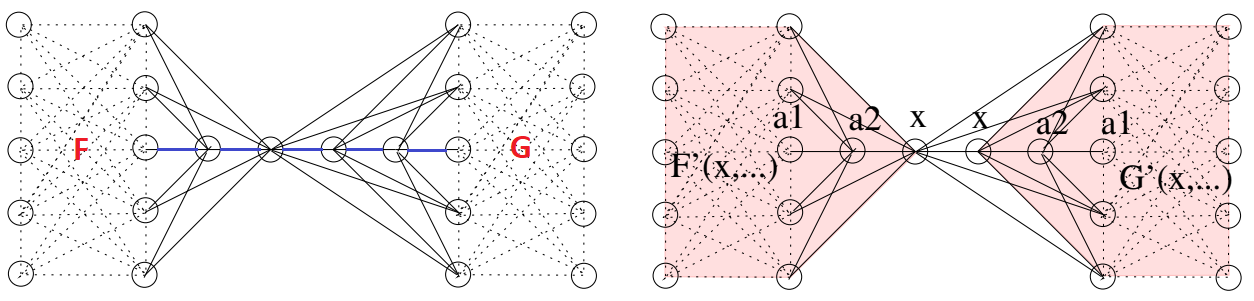
\includegraphics[width=\textwidth]{images/PostAlg.png}
	\caption{A graphical representation of the postprocessing algorithm involving two general penalty functions (F and G) linked by a chain (blue edges). It is important to notice the swap of role between the original node representing the shared variable to ensure consistency of the variable's value between functions.}
	\end{center}
\end{figure}
Post-processing cannot be applied to every quantum architecture. In order to be successful, it is necessary that qubits presents an high numbers of connections with other qubits. If this condition is not satisfied, we will not obtain great results from the re-computation of scores for penalty functions: nodes belonging to the chain will not link with external qubits and no new couplings to consider will emerge. D-Wave currently proposes two main architectures: the older one, Chimera, is clearly affected by this issue. Actually he graph of its nodes is sparse and a qubits has at most 6 neighbour qubits. On the other hand the most recent architecture, Pegasus, is less sparse and it usually does not fall into the issue described above. As a consequence, from now on we will assume that the algorithm will be executed only on the Pegasus architecture.


\section{Implementation}

While the definition of the approach is linear, in practice we have to deal with numerous issues, mainly caused by computational constraints. As a consequence, the implementation relies on some heuristic that avoid apparent deadlock point during execution.
The workflow of the implementation is shown in figure 4.2.
More details on each step will be provided in the next paragraphs.

\begin{figure}[t]
	\begin{center}
	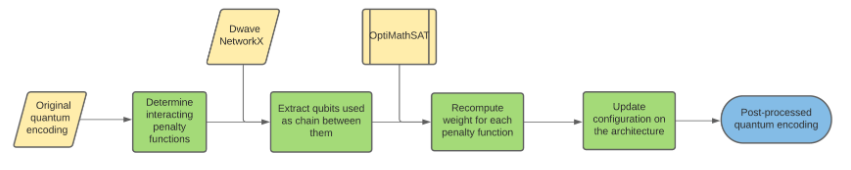
\includegraphics[width=\textwidth]{images/Workflow.png}
	\caption{A graphical representation of the workflow necessary to implement the postprocessing algorithm. Yellow nodes represent data and state-of-the-art tools; green nodes represent tasks implemented in this thesis.}
	\end{center}
\end{figure}

\subsection{Extracting encoding information}

The original version of the code returned the list of values assigned to each parameter, without any additional information about the mapping between Boolean sub-formulas and qubits. While it was not relevant in the precedent version, obtaining this information is now essential to determine how to rearrange qubits in new penalty functions. \\
To solve the issue, it was required to modify the \textit{place\_and\_route} library and collect data from the intermediate steps of the procedure. [Continue]

\subsection{Re-assigning qubits}

Once the needed data are stored and available, we can start to post-process the original encoding determining what functions might be extended and what chains are involved. For each pair of penalty functions we decide if there is a chain connecting them which can be split in two disjoint sub-sets of qubits without altering the correctness of the encoding of the original formula.

\subsection{Recomputing penalty functions}

In order to generate the OMT instance necessary to recompute the parameters on the enhanced penalty functions, we need to build the quadruplets of data necessary and call the \textit{searchPF} function using them.\\
We also tried to enhance the actual encoding, modifying the definition of the SMT file. 

\subsection{Updating the configuration}

\newpage

